
از وبسایت وبتون چپتر هارا دانلود میکنیم و در هر صفحه OCR را اجرا میکنیم و متن هر چپتر را استخراج میکنیم و در فرمت  [chapter\_title].txt ذخیره میکنیم.
\\
از آنجایی که در NER نقش واژه ها اهمیت دارد. جمله های تک واژه ای را حذف میکنیم و  سپس به کمک ابزار ntlk و تابع sent\_tokenize جملات را تشخیص میدهیم.
\\
حال جملات را با کمک این ابزار برچسب گذاری میکنیم.
 \begin{latin}
 \url{https://tecoholic.github.io/ner-annotator}
 \end{latin}
\\
در این ابزار از جملاتی که تگ ندارند، skip میکنیم بنابراین در داده تمیز شده حذف میشوند.
\\
و سپس تمام متن های تمیز شده چپتر ها را با برچسب هایشان به صورت فایل csv ذخیره میکنیم.



أ. تعداد «واحد» داده
\begin{latin}
\begin{center}
  \fontsize{8pt}{9pt}\ttfamily
  \csvautotabular[respect all]{../stats/data_count.csv}
\end{center}
\end{latin}

\\
ب. تعداد جملات
\begin{latin}
\begin{center}
  \fontsize{8pt}{9pt}\ttfamily
  \csvautotabular[respect all]{../stats/sentences_count.csv}
\end{center}
\end{latin}

\\
\newpage
ج. تعداد کلمات
\begin{latin}
\begin{center}
  \fontsize{8pt}{9pt}\ttfamily
  \csvautotabular[respect all]{../stats/words_count.csv}
\end{center}
\end{latin}

\\

د. تعداد کلمات منحصر به فرد

\

\begin{latin}
\begin{center}
  \fontsize{8pt}{9pt}\ttfamily
  \csvautotabular[respect all]{../stats/unique_common_uncommon_count.csv}
\end{center}
\end{latin}

ه. تعداد کلمات منحصر به فرد مشترک و غیر مشترک بین برچسب ها
\begin{latin}
\begin{center}
  \fontsize{8pt}{9pt}\ttfamily
  \csvautotabular[respect all]{../stats/unique_common_uncommon_count.csv}
\end{center}
\end{latin}

\newpage

و.  ۱۰کلمه پرتکرار غیر مشترک هر برچسب
\begin{latin}
\begin{center}
    \fontsize{4pt}{7pt}\ttfamily
  \csvautotabular[respect all]{../stats/ten_uncommon_words.csv}
\end{center}
\end{latin}

ز.  ۱۰کلمه مشترک برتر هر برچسب نسبت به برچسبهای دیگر بر اساس معیار زیر
\begin{latin}
\begin{center}
  \fontsize{4pt}{7pt}\ttfamily
  \csvautotabular[respect all]{../stats/ten_common_words.csv}
\end{center}
\end{latin}


ح. ده کلمه برتر بر اساس \lr{TF\_IDF(W)}
\begin{latin}
\begin{center}
  \fontsize{4pt}{7pt}\ttfamily
  \csvautotabular[respect all]{../stats/ten_common_words.csv}
\end{center}
\end{latin}


\newpage

ط. هیستوگرام تعداد تکرار هر کلمه منحصر به فرد به ترتیب از فرکانس بالا به پایین
\begin{figure}[H]
    \centering
    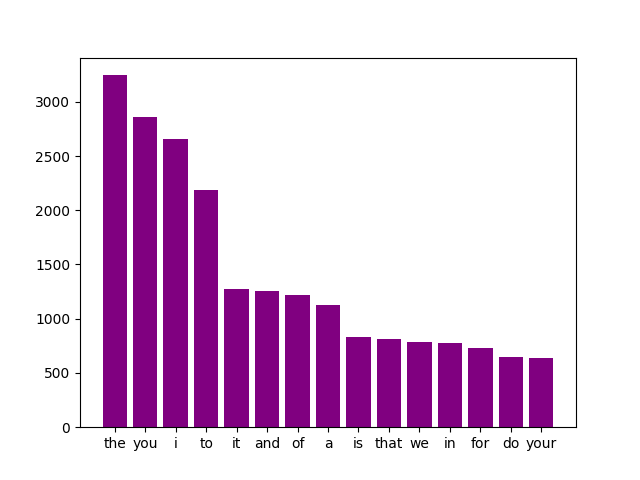
\includegraphics[width=0.7\linewidth]{../stats/hist.png}
   \end{figure}
   
لینک \lr{github} :
\\
 \begin{latin}
 \url{https://github.com/Bayany/NLP_NER}
 \end{latin}
 

\\
لینک \lr{huggingface}:
\\
 \begin{latin}
 \url{https://huggingface.co/datasets/Bayany/NER}
 \end{latin}
 
